% =============================================================================
%  StructureTower 数論シリーズ（NT3）
%  塔比較理論（Tower Comparison Theory）
%  LuaLaTeX 文書
% =============================================================================
\documentclass[a4paper,11pt]{ltjsarticle}

%% ─── パッケージ ─────────────────────────────────────────────────────────────
\usepackage{luatexja-fontspec}
\usepackage{amsmath,amssymb,amsthm,mathtools}
\usepackage{tikz-cd}
\usepackage{tikz}
\usetikzlibrary{arrows.meta,positioning,calc,decorations.pathmorphing,matrix}
\usepackage{enumitem}
\usepackage{hyperref}
\usepackage{tcolorbox}
\tcbuselibrary{skins,breakable}
\usepackage{listings}
\usepackage{xcolor}
\usepackage{geometry}
\usepackage{fancyhdr}
\usepackage{float}
\usepackage{bm}

%% ─── ページ設定 ──────────────────────────────────────────────────────────────
\geometry{margin=2.5cm, top=3cm, bottom=3cm}

%% ─── フォント ────────────────────────────────────────────────────────────────
\setmainjfont{Harano Aji Mincho}[
  BoldFont = Harano Aji Mincho,
  BoldFeatures = {FakeBold=2},
]
\setsansjfont{Harano Aji Gothic}
\setmonofont[Scale=0.85]{DejaVu Sans Mono}

%% ─── 色 ──────────────────────────────────────────────────────────────────────
\definecolor{leanblue}{HTML}{2563EB}
\definecolor{leanbg}{HTML}{F8FAFC}
\definecolor{leancomment}{HTML}{6B7280}
\definecolor{leankeyword}{HTML}{7C3AED}
\definecolor{leanstring}{HTML}{059669}
\definecolor{accentcolor}{HTML}{1E40AF}
\definecolor{theoremcolor}{HTML}{EFF6FF}
\definecolor{definitioncolor}{HTML}{F0FDF4}
\definecolor{remarkcolor}{HTML}{FFF7ED}
\definecolor{ringcolor}{HTML}{FEF2F2}
\definecolor{groupcolor}{HTML}{F0F9FF}

%% ─── hyperref ────────────────────────────────────────────────────────────────
\hypersetup{
  colorlinks=true,
  linkcolor=accentcolor,
  urlcolor=leanblue,
  citecolor=accentcolor,
  pdftitle={StructureTower NT3：塔比較理論},
  pdfauthor={su},
}

%% ─── 定理環境 ────────────────────────────────────────────────────────────────
\theoremstyle{definition}
\newtheorem{definition}{定義}[section]
\newtheorem{example}[definition]{例}
\newtheorem{exercise}[definition]{演習}

\theoremstyle{plain}
\newtheorem{theorem}[definition]{定理}
\newtheorem{lemma}[definition]{補題}
\newtheorem{proposition}[definition]{命題}
\newtheorem{corollary}[definition]{系}

\theoremstyle{remark}
\newtheorem{remark}[definition]{注意}

%% ─── tcolorbox スタイル ───────────────────────────────────────────────────────
\newtcolorbox{proofstrategy}{
  colback=remarkcolor,
  colframe=orange!60!black,
  title={\textbf{証明戦略}},
  fonttitle=\sffamily,
  boxrule=0.5pt,
  arc=3pt,
}

\newtcolorbox{mathinsight}{
  colback=theoremcolor,
  colframe=accentcolor,
  title={\textbf{数学的洞察}},
  fonttitle=\sffamily,
  boxrule=0.5pt,
  arc=3pt,
}

\newtcolorbox{maintheorem}{
  colback=definitioncolor,
  colframe=green!50!black,
  title={\textbf{主定理}},
  fonttitle=\sffamily,
  boxrule=0.8pt,
  arc=3pt,
}

%% ─── Lean コードリスト ────────────────────────────────────────────────────────
\lstdefinelanguage{lean4}{
  morekeywords={def,theorem,lemma,example,instance,class,structure,
    where,let,in,do,if,then,else,match,with,fun,return,
    import,open,namespace,section,end,variable,
    inductive,abbrev,noncomputable,private,protected,
    sorry,admit,have,show,suffices,calc,by,exact,
    apply,intro,intros,constructor,cases,induction,
    simp,rw,rfl,ext,ring,linarith,omega,norm_num,
    decide,trivial,assumption,contradiction,classical,
    refine,rcases,obtain,use,push_neg,funext,
    Type,Prop,Sort,Set,true,false,
    attribute,deriving},
  sensitive=true,
  morecomment=[l]{--},
  morecomment=[n]{/-}{-/},
  morestring=[b]",
  literate=
    {α}{{\(\alpha\)}}1
    {β}{{\(\beta\)}}1
    {γ}{{\(\gamma\)}}1
    {ι}{{\(\iota\)}}1
    {κ}{{\(\kappa\)}}1
    {σ}{{\(\sigma\)}}1
    {τ}{{\(\tau\)}}1
    {φ}{{\(\varphi\)}}1
    {δ}{{\(\delta\)}}1
    {→}{{\(\to\)}}1
    {←}{{\(\leftarrow\)}}1
    {↔}{{\(\leftrightarrow\)}}1
    {⟨}{{\(\langle\)}}1
    {⟩}{{\(\rangle\)}}1
    {≤}{{\(\leq\)}}1
    {≥}{{\(\geq\)}}1
    {≠}{{\(\neq\)}}1
    {∀}{{\(\forall\)}}1
    {∃}{{\(\exists\)}}1
    {∧}{{\(\wedge\)}}1
    {∨}{{\(\vee\)}}1
    {¬}{{\(\neg\)}}1
    {∈}{{\(\in\)}}1
    {∉}{{\(\notin\)}}1
    {⊆}{{\(\subseteq\)}}1
    {⊂}{{\(\subset\)}}1
    {∪}{{\(\cup\)}}1
    {∩}{{\(\cap\)}}1
    {⋂}{{\(\bigcap\)}}1
    {⋃}{{\(\bigcup\)}}1
    {∅}{{\(\emptyset\)}}1
    {×}{{\(\times\)}}1
    {∘}{{\(\circ\)}}1
    {ℕ}{{\(\mathbb{N}\)}}1
    {ℤ}{{\(\mathbb{Z}\)}}1
    {ℝ}{{\(\mathbb{R}\)}}1
    {ℚ}{{\(\mathbb{Q}\)}}1
    {:=}{{:=}}2,
}

\lstset{
  language=lean4,
  basicstyle=\ttfamily\small,
  keywordstyle=\color{leankeyword}\bfseries,
  commentstyle=\color{leancomment}\itshape,
  stringstyle=\color{leanstring},
  backgroundcolor=\color{leanbg},
  frame=single,
  rulecolor=\color{gray!30},
  xleftmargin=1em,
  xrightmargin=0.5em,
  breaklines=true,
  breakatwhitespace=true,
  keepspaces=true,
  columns=flexible,
  showstringspaces=false,
}

%% ─── ヘッダー・フッター ──────────────────────────────────────────────────────
\pagestyle{fancy}
\fancyhf{}
\fancyhead[L]{\small\sffamily StructureTower NT3：塔比較理論}
\fancyhead[R]{\small\sffamily su}
\fancyfoot[C]{\thepage}
\renewcommand{\headrulewidth}{0.4pt}

%% ─── マクロ ──────────────────────────────────────────────────────────────────
\newcommand{\ST}{\mathsf{ST}}
\newcommand{\level}[2]{#1.\mathrm{level}(#2)}
\newcommand{\NatInc}{\sqsubseteq}
\newcommand{\towerMeet}{\sqcap}
\newcommand{\towerJoin}{\sqcup}
\newcommand{\reindex}{\mathrm{reindex}}
\newcommand{\union}{\mathrm{union}}
\newcommand{\glob}{\mathrm{global}}
\newcommand{\Hom}{\mathrm{Hom}}
\newcommand{\map}{\mathrm{map}}
\newcommand{\comap}{\mathrm{comap}}
\newcommand{\Dev}{\delta}        % deviation map
\newcommand{\OD}{\mathbb{N}^{\mathrm{op}}}

% =============================================================================
\begin{document}
% =============================================================================

%% ─── タイトル ────────────────────────────────────────────────────────────────
\title{%
  \textbf{StructureTower 数論シリーズ NT3}\\[0.3em]
  \large 塔比較理論（Tower Comparison Theory）}
\author{su}
\date{2026年3月}
\maketitle

%% ─── AI disclosure ───────────────────────────────────────────────────────────
\begin{center}
\small
\textit{AI assistance disclosure:}
Lean ソースコードは Claude (Anthropic) で骨格を生成し、
Codex (OpenAI) で修正した。
\TeX 文書は Claude Code (Anthropic) で生成した。
著者による加筆・修正は行っていない。
内容の正確性は保証されず、誤りがあれば著者の責任である。
\end{center}

\begin{abstract}
本稿は Lean~4 / Mathlib4 上で形式化された StructureTower 数論シリーズの第3回として、
\textbf{塔比較理論（Tower Comparison Theory）}を解説する。
NT1 で構築した分岐群塔（ramification tower）と NT2 で導入した
上付番号変換（Herbrand upper numbering）を統合し、
異なる型上の StructureTower を結ぶ写像構造を体系化する。
主要な概念として、交差塔・和塔（§1）、TowerPairing（§2）、
環-群二重塔データ（§3）、Reindex 整合的対（§4）、そして
偏差写像による数論的統合（§5）を順に論じる。
最終的には「群の塔が環の塔から偏差写像を通じて完全に決定される」
という主定理候補（Tower Duality 定理）に到達する。
\end{abstract}

\tableofcontents
\newpage

% =============================================================================
\section{はじめに：塔比較の問題設定}
% =============================================================================

\subsection{NT1-NT2 の振り返り}

NT1 では、局所体の分岐理論における基本構造である\textbf{分岐群列}を
StructureTower として定式化した。
群 $G$（ガロア群）の正規部分群の減少列
\[
G = G_0 \supseteq G_1 \supseteq G_2 \supseteq \cdots
\]
は \texttt{ramificationTower} として \(\ST(\OD, G)\) の元となる。

NT2 では、Herbrand の上付番号付け（upper numbering）を \texttt{reindex} として定式化した。
スケーリング関数 \(\varphi : \mathbb{N} \to \mathbb{N}\)（\texttt{scaledHerbrand}）による
塔の再添字付けが \texttt{upperNumberingTower} を与える。

\subsection{NT3 の核心的問い}

\begin{mathinsight}
2つの異なる型 $\alpha$, $\beta$ 上の $\ST(T_1)$, $\ST(T_2)$ が
同じ添字集合 $\iota$ を共有するとき、それらの間にどのような
\textbf{比較構造}が成り立ちうるか？
\end{mathinsight}

より具体的には：
\begin{itemize}
  \item 環の塔 \(T_R : \ST(\OD, R)\)（イデアル冪塔）と
        群の塔 \(T_G : \ST(\OD, G)\)（分岐群塔）は
        どのように「同じ算術を記述している」と言えるか？
  \item Herbrand の reindex を 2つの塔に同時に適用したとき、
        整合性はどのように定式化できるか？
\end{itemize}

これらの問いに答えるために、NT3 では Tower Comparison Theory の基礎を整備する。

% =============================================================================
\section{\S NT3-1：塔の交差と積}
% =============================================================================

\subsection{同一型上の2塔の比較}

2つの塔 $T_1, T_2 : \ST(\iota, \alpha)$ が同一型 $\alpha$ 上で与えられたとき、
最も基本的な比較は\textbf{レベルごとの集合演算}による新しい塔の構成である。

\begin{definition}[交差塔・和塔]
添字順序集合 $(\iota, \leq)$ と $T_1, T_2 : \ST(\iota, \alpha)$ に対し、
\begin{align}
  (T_1 \towerMeet T_2).\mathrm{level}(i) &:= T_1.\mathrm{level}(i) \cap T_2.\mathrm{level}(i), \\
  (T_1 \towerJoin T_2).\mathrm{level}(i) &:= T_1.\mathrm{level}(i) \cup T_2.\mathrm{level}(i).
\end{align}
いずれも単調性を継承し、StructureTower となる。
\end{definition}

\begin{remark}
交差塔が well-defined であることは直ちに分かる（$\cap$ の単調性）。
和塔についても $\cup$ の単調性から成立する。
すなわち $x \in T_1.\mathrm{level}(i) \cup T_2.\mathrm{level}(i)$ かつ $i \leq j$ なら
$x \in T_1.\mathrm{level}(j) \cup T_2.\mathrm{level}(j)$。
\end{remark}

\subsection{NatInclusion の半順序構造}

\begin{definition}[NatInclusion]
$T, T' : \ST(\iota, \alpha)$ に対し、
\[
T \NatInc T' \iff \forall i,\; T.\mathrm{level}(i) \subseteq T'.\mathrm{level}(i).
\]
\end{definition}

$\NatInc$ は $\ST(\iota, \alpha)$ 上の前順序（実際は半順序）を与える。

\begin{proposition}[交差塔は最大下界]
$T_1, T_2, T : \ST(\iota, \alpha)$ に対し、
\[
T \NatInc (T_1 \towerMeet T_2) \iff T \NatInc T_1 \wedge T \NatInc T_2.
\]
すなわち $T_1 \towerMeet T_2$ は $\NatInc$ による最大下界（infimum）である。
\end{proposition}

\begin{proof}
$(\Rightarrow)$: 交差塔の定義より $T_1 \towerMeet T_2 \NatInc T_1$ かつ
$T_1 \towerMeet T_2 \NatInc T_2$ だから、推移律による。\\
$(\Leftarrow)$: 各 $i$ と $x \in T.\mathrm{level}(i)$ に対し、
$x \in T_1.\mathrm{level}(i)$ かつ $x \in T_2.\mathrm{level}(i)$ だから
$x \in T_1.\mathrm{level}(i) \cap T_2.\mathrm{level}(i)$。\hfill$\square$
\end{proof}

\subsection{global との整合性}

\begin{proposition}[global の交差分配]
\[
\glob(T_1 \towerMeet T_2) = \glob(T_1) \cap \glob(T_2).
\]
\end{proposition}

\begin{proof}
$\glob(T) = \bigcap_i T.\mathrm{level}(i)$ の定義と、任意積と交差の交換可能性
$\bigcap_i (A_i \cap B_i) = (\bigcap_i A_i) \cap (\bigcap_i B_i)$
から直ちに従う。\hfill$\square$
\end{proof}

\begin{figure}[h]
\centering
\begin{tikzpicture}[
  tower/.style={draw, rounded corners=3pt, minimum width=2.2cm, minimum height=0.7cm, align=center},
  arrow/.style={-Stealth, thick},
  natinc/.style={dashed, -Stealth, gray}
]
% T1
\node[tower, fill=blue!10] (T1) at (0,0) {$T_1$};
% T2
\node[tower, fill=red!10]  (T2) at (3,0) {$T_2$};
% meet
\node[tower, fill=purple!10] (M) at (1.5,-2) {$T_1 \towerMeet T_2$};
% join
\node[tower, fill=green!10]  (J) at (1.5,2) {$T_1 \towerJoin T_2$};
% T
\node[tower, fill=gray!10]   (T) at (-2,-2) {$T$};

\draw[natinc] (M) -- node[right,font=\small]{$\NatInc$} (T1);
\draw[natinc] (M) -- node[left,font=\small]{$\NatInc$} (T2);
\draw[natinc] (T1) -- node[left,font=\small]{$\NatInc$} (J);
\draw[natinc] (T2) -- node[right,font=\small]{$\NatInc$} (J);
\draw[arrow] (T) -- node[above,font=\small]{$\NatInc T_1$} (T1);
\draw[arrow] (T) -- node[below,font=\small,sloped]{$\NatInc T_2$} (T2);
\draw[arrow,dashed,blue!60!black,thick] (T) -- node[left,font=\small]{$\NatInc$} (M);

\node[font=\small\itshape, gray] at (1.5,-3.2) {交差塔は NatInclusion の infimum};
\end{tikzpicture}
\caption{$T_1 \towerMeet T_2$ が $\NatInc$ の最大下界であることを示すハッセ図（略図）。
$T \NatInc T_1$ かつ $T \NatInc T_2$ ならば $T \NatInc T_1 \towerMeet T_2$。}
\end{figure}

% =============================================================================
\section{\S NT3-2：TowerPairing}
% =============================================================================

\subsection{異なる型の塔を結ぶ}

$T_1 : \ST(\iota, \alpha)$ と $T_2 : \ST(\iota, \beta)$ を
\textbf{異なる型}上の塔とする。
両者を結ぶ基本的な概念は Hom である。

\begin{definition}[StructureTower Hom]
\[
\Hom(T_1, T_2) = \bigl\{ f : \alpha \to \beta \;\big|\;
  \forall i,\; f(T_1.\mathrm{level}(i)) \subseteq T_2.\mathrm{level}(i) \bigr\}.
\]
\end{definition}

しかし Hom は一方向の写像にすぎない。
「2つの塔が同じ情報を符号化している」という双方向の関係を捉えるには：

\begin{definition}[TowerPairing]
$T_1 : \ST(\iota, \alpha)$, $T_2 : \ST(\iota, \beta)$ に対し、
\textbf{TowerPairing} とは以下からなるデータである：
\begin{itemize}
  \item 前方射 $f : \alpha \to \beta$（$f \in \Hom(T_1, T_2)$）
  \item 後方射 $g : \beta \to \alpha$（$g \in \Hom(T_2, T_1)$）
\end{itemize}
すなわち $f$ と $g$ の両方が対応するレベルを保存する。
\end{definition}

\begin{remark}
TowerPairing は同型よりも弱い条件である。
$f \circ g = \mathrm{id}$ や $g \circ f = \mathrm{id}$ は要求しない。
これはガロア対応の「前方射：制限」「後方射：埋め込み」の抽象版である。
\end{remark}

\subsection{map と comap との関係}

\begin{proposition}[map/comap と NatInclusion の同値性]
$f : \alpha \to \beta$ と $T_1 : \ST(\iota, \alpha)$,
$T_2 : \ST(\iota, \beta)$ に対し、
\begin{align}
  f \in \Hom(T_1, T_2) &\iff \map(f, T_1) \NatInc T_2, \\
  f \in \Hom(T_1, T_2) &\iff T_1 \NatInc \comap(f, T_2).
\end{align}
ここで $\map(f, T).\mathrm{level}(i) = f(T.\mathrm{level}(i))$,
$\comap(f, T).\mathrm{level}(i) = f^{-1}(T.\mathrm{level}(i))$。
\end{proposition}

\begin{figure}[h]
\centering
\begin{tikzcd}[column sep=4cm, row sep=1.5cm]
\ST(\iota, \alpha) \arrow[r, "\map(f{,}\cdot)", bend left=15]
  \arrow[d, "\NatInc"', dashed]
&
\ST(\iota, \beta) \arrow[d, "\NatInc", dashed]
  \arrow[l, "\comap(f{,}\cdot)", bend left=15]
\\
T_1 \arrow[r, "f \in \Hom", swap]
&
T_2
\end{tikzcd}
\caption{$\map$ と $\comap$ の対称性。$\map(f, T_1) \NatInc T_2 \iff T_1 \NatInc \comap(f, T_2)$
はガロア接続（Galois connection）の構造を持つ。}
\end{figure}

\subsection{TowerPairing の圏論的性質}

\begin{proposition}[恒等と合成]
\leavevmode
\begin{enumerate}
  \item 任意の $T : \ST(\iota, \alpha)$ に対し、
        恒等 TowerPairing $\mathrm{id}_T$ が存在する（$f = g = \mathrm{id}$）。
  \item $p : \mathrm{TP}(T_1, T_2)$ と $q : \mathrm{TP}(T_2, T_3)$ があれば、
        合成 $q \circ p : \mathrm{TP}(T_1, T_3)$ が存在する
        （前方射：$q.f \circ p.f$、後方射：$p.g \circ q.g$）。
\end{enumerate}
\end{proposition}

\begin{figure}[h]
\centering
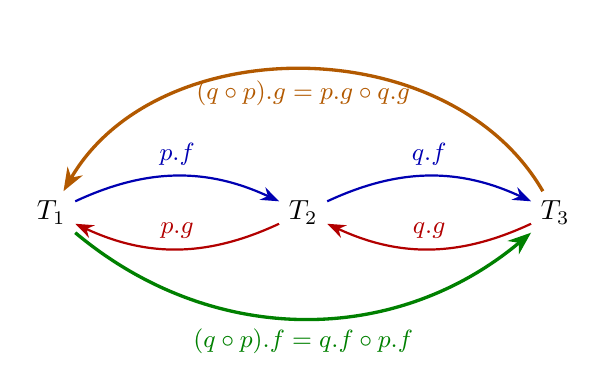
\begin{tikzpicture}[node distance=3.2cm, auto]
\node (A) {$T_1$};
\node (B) [right of=A] {$T_2$};
\node (C) [right of=B] {$T_3$};

\draw[-Stealth, thick, blue!70!black, bend left=25] (A) to
  node[above, font=\small]{$p.f$} (B);
\draw[-Stealth, thick, red!70!black, bend left=25] (B) to
  node[above, font=\small]{$p.g$} (A);
\draw[-Stealth, thick, blue!70!black, bend left=25] (B) to
  node[above, font=\small]{$q.f$} (C);
\draw[-Stealth, thick, red!70!black, bend left=25] (C) to
  node[above, font=\small]{$q.g$} (B);

\draw[-Stealth, very thick, green!50!black, bend right=40] (A) to
  node[below, font=\small]{$(q\circ p).f = q.f\circ p.f$} (C);
\draw[-Stealth, very thick, orange!70!black, bend right=60] (C) to
  node[below, font=\small]{$(q\circ p).g = p.g\circ q.g$} (A);
\end{tikzpicture}
\caption{TowerPairing の合成。前方射は通常の関数合成、後方射は逆順の合成になる点に注意。}
\end{figure}

% =============================================================================
\section{\S NT3-3：誘導塔と環-群二重フィルトレーション}
% =============================================================================

\subsection{双対塔対の動機}

NT1-\S5 で見た構造を振り返る：
\begin{itemize}
  \item \textbf{環側}：イデアル冪塔 $T_R = \mathrm{idealPowTower}(I) : \ST(\OD, R)$
  \item \textbf{群側}：分岐群塔 $T_G = \mathrm{ramificationTower}(rd) : \ST(\OD, G)$
  \item \textbf{橋}：群 $G$ が $R$ に環自己同型として作用し、各 $\sigma \in G_n$ が
        $I^n$ 上で「恒等的に」作用する
\end{itemize}

この「橋」の役割を果たすのが\textbf{偏差写像}（deviation map）である：
\[
\delta_\sigma : R \to R, \quad x \mapsto \sigma(x) - x.
\]
$\sigma \in G_n$ ならば $\delta_\sigma(x) \in I^n$（整合条件）。

\subsection{RingGroupTowerData}

\begin{definition}[環-群二重塔データ]
\texttt{RingGroupTowerData} は以下からなる：
\begin{itemize}
  \item 可換環 $R$ と部分群の反単調列 $G_0 \supseteq G_1 \supseteq \cdots$ を持つ群 $G$
  \item イデアル $I \trianglelefteq R$
  \item 群作用 $\sigma \mapsto (\sigma : R \xrightarrow{\sim} R)$
  \item \textbf{整合条件}：$\sigma \in G_n \Rightarrow \forall x \in R,\; \delta_\sigma(x) \in I^n$
\end{itemize}
ここから環側の塔 $T_R = \mathrm{idealPowTower}(I)$ と
群側の塔 $T_G$ が自然に得られる。
\end{definition}

\begin{figure}[h]
\centering
\begin{tikzpicture}[
  level/.style={rectangle, draw, rounded corners=2pt, minimum width=2cm, minimum height=0.5cm, font=\small},
  >=Stealth
]
% 環側の塔
\node[level, fill=red!10] (R0) at (0,3.5) {$R = I^0$};
\node[level, fill=red!15] (R1) at (0,2.5) {$I^1$};
\node[level, fill=red!20] (R2) at (0,1.5) {$I^2$};
\node[level, fill=red!25] (R3) at (0,0.5) {$I^3$};
\node at (0,-0.3) {$\vdots$};
\node[font=\small\bfseries] at (0,4.3) {環の塔 $T_R$};

\draw[thick] (R0.south) -- (R1.north);
\draw[thick] (R1.south) -- (R2.north);
\draw[thick] (R2.south) -- (R3.north);

% 群側の塔
\node[level, fill=blue!10] (G0) at (5,3.5) {$G_0 = G$};
\node[level, fill=blue!15] (G1) at (5,2.5) {$G_1$};
\node[level, fill=blue!20] (G2) at (5,1.5) {$G_2$};
\node[level, fill=blue!25] (G3) at (5,0.5) {$G_3$};
\node at (5,-0.3) {$\vdots$};
\node[font=\small\bfseries] at (5,4.3) {群の塔 $T_G$};

\draw[thick] (G0.south) -- (G1.north);
\draw[thick] (G1.south) -- (G2.north);
\draw[thick] (G2.south) -- (G3.north);

% 偏差写像による橋
\foreach \n/\y in {0/3.5, 1/2.5, 2/1.5, 3/0.5} {
  \draw[-Stealth, dashed, thick, green!60!black]
    (G\n.west) -- node[above, font=\tiny]{$\delta_\sigma$} (R\n.east);
}

% 整合条件の注記
\node[draw, rounded corners=3pt, fill=green!5, font=\small, align=center] at (2.5,-1.2)
  {整合条件：$\sigma \in G_n \Rightarrow \delta_\sigma(R) \subseteq I^n$};
\end{tikzpicture}
\caption{環-群二重塔の構造。群の塔の各レベル $G_n$ の元 $\sigma$ による偏差 $\delta_\sigma(x) = \sigma(x)-x$
は、対応する環の塔のレベル $I^n$ に収まる（整合条件）。}
\end{figure}

\subsection{偏差写像の加法性}

\begin{proposition}[偏差の telescoping 恒等式]
群元の積に対し、偏差写像は以下の恒等式を満たす：
\[
\delta_{\sigma\tau}(x) = \delta_\sigma(\tau(x)) + \delta_\tau(x).
\]
\end{proposition}

\begin{proof}
直接計算による：
\[
(\sigma\tau)(x) - x = \bigl(\sigma(\tau(x)) - \tau(x)\bigr) + \bigl(\tau(x) - x\bigr)
= \delta_\sigma(\tau(x)) + \delta_\tau(x). \quad \square
\]
\end{proof}

\begin{remark}[交換子条件への応用]
この telescoping 恒等式は、分岐群の交換子条件
$[G_i, G_j] \subseteq G_{i+j}$ の根拠となる重要な等式である。
$\sigma \in G_i$, $\tau \in G_j$ のとき、
交換子 $[\sigma, \tau] = \sigma^{-1}\tau^{-1}\sigma\tau$ の偏差が
$I^{i+j}$ に入ることが、この式から導かれる。
\end{remark}

% =============================================================================
\section{\S NT3-4：Reindex 整合的対}
% =============================================================================

\subsection{一般化の動機}

NT2 で見た Hasse-Arf 定理の本質は、
「Herbrand の reindex \(\varphi\) が部分群への制限と整合する」ことであった。
これを一般的な枠組みで定式化する。

\begin{definition}[Reindex 整合条件]
$T_1 : \ST(\iota, \alpha)$, $T_2 : \ST(\iota, \beta)$,
$f : \alpha \to \beta$,
$\varphi_1, \varphi_2 : \iota \to \iota$（単調）に対し、
\[
\mathrm{IsReindexCompatible}(T_1, T_2, f, \varphi_1, \varphi_2)
\iff \forall i,\; f\bigl(T_1.\mathrm{level}(\varphi_1(i))\bigr)
   \subseteq T_2.\mathrm{level}(\varphi_2(i)).
\]
\end{definition}

\begin{proposition}[特殊ケース]
\leavevmode
\begin{enumerate}
  \item $\varphi_1 = \varphi_2 = \mathrm{id}$ のとき、通常の Hom 条件に帰着する：
        \[
        \mathrm{IsReindexCompatible}(T_1, T_2, f, \mathrm{id}, \mathrm{id})
        \iff f \in \Hom(T_1, T_2).
        \]
  \item 合成則：$f$ が $(T_1, \varphi_1) \to (T_2, \varphi_2)$ に、
        $g$ が $(T_2, \varphi_2) \to (T_3, \varphi_3)$ にそれぞれ整合的なら、
        $g \circ f$ は $(T_1, \varphi_1) \to (T_3, \varphi_3)$ に整合的。
\end{enumerate}
\end{proposition}

\subsection{NT2 の Herbrand 整合性の一般化}

\begin{figure}[h]
\centering
\begin{tikzcd}[row sep=2.5cm, column sep=3.5cm]
\ST(\OD, G) \arrow[r, "\reindex(\varphi_G)"] \arrow[d, "\text{制限}"]
& \ST(\OD, G) \arrow[d, "\text{制限}"] \\
\ST(\OD, H) \arrow[r, "\reindex(\varphi_H)"]
& \ST(\OD, H)
\end{tikzcd}
\caption{Herbrand upper numbering の整合性（NT2 の UpperNumberingCompatible の概念図）。
図式が可換になるのは $\varphi_G$ と $\varphi_H$ が「整合的」に選ばれているときである。}
\end{figure}

NT2 における \texttt{UpperNumberingCompatible} は、
$T_1 = \mathrm{ramificationTower}(G)$,
$T_2 = \mathrm{ramificationTower}(H)$ (部分群 $H \leq G$ 上),
$f = H \hookrightarrow G$ の包含写像,
$\varphi_1 = \mathrm{herbrandReindex}(G)$,
$\varphi_2 = \mathrm{herbrandReindex}(H)$
として \texttt{IsReindexCompatible} の特殊ケースである。

% =============================================================================
\section{\S NT3-5：数論的統合と主定理}
% =============================================================================

\subsection{IsExactPairing}

\begin{definition}[Exact Pairing]
$d : \mathrm{RingGroupTowerData}(R, G)$ に対し、
$d$ が \textbf{exact} であるとは：
\[
\mathrm{IsExactPairing}(d) \iff \forall n,\;
\bigl(d.G_n : \text{Set}~G\bigr) =
\bigl\{\sigma \in G \;\big|\; \forall x \in R,\; \delta_\sigma(x) \in I^n\bigr\}.
\]
すなわち、群の塔のレベルが偏差条件によって\textbf{完全に特徴付けられる}。
\end{definition}

\begin{remark}
Exact でない場合は $G_n$ が偏差条件より「広い」ことがある
（$G_n \supseteq \{\sigma \mid \forall x, \delta_\sigma(x) \in I^n\}$）。
整合条件は常に $G_n \subseteq $ （偏差条件集合）を与えるが、
逆向きは exactness の仮定が必要。
\end{remark}

\subsection{ジャンプ集合と環-群対応}

\begin{definition}[ジャンプ集合]
$T : \ST(\OD, \alpha)$ に対し、\textbf{ジャンプ集合}を
\[
\mathrm{jumpSet}(T) := \bigl\{n \in \mathbb{N} \;\big|\;
T.\mathrm{level}(n) \setminus T.\mathrm{level}(n+1) \neq \emptyset\bigr\}
\]
と定義する。これは「塔が n と n+1 の間で『ジャンプ』するレベルの集合」である。
\end{definition}

\begin{proposition}[ジャンプ集合の特徴付け]
$\mathrm{IsExactPairing}(d)$ のもとで、
\[
n \in \mathrm{jumpSet}(d.T_G) \iff
\exists \sigma \in G,\; \sigma \in G_n \wedge \sigma \notin G_{n+1}.
\]
\end{proposition}

\subsection{主定理候補：Tower Duality}

\begin{maintheorem}[Tower Duality（候補）]
$d : \mathrm{RingGroupTowerData}(R, G)$ が $\mathrm{IsExactPairing}$ を満たすとき、
群の塔 $d.T_G$ は環の塔 $d.T_R$ から偏差写像 $\delta$ を通じて
\textbf{完全に決定される}：
\[
d.G_n = \bigl\{\sigma \in G \;\big|\; \forall x \in R,\; \delta_\sigma(x) \in I^n\bigr\}.
\]
さらに、Herbrand reindex $\varphi$ が \texttt{IsReindexCompatible} を満たすならば、
上付番号塔 \texttt{upperNumberingTower} も環の塔から決定される。
\end{maintheorem}

\begin{figure}[h]
\centering
\begin{tikzpicture}[
  >=Stealth,
  box/.style={draw, rounded corners=4pt, minimum width=3cm, minimum height=1cm, align=center, font=\small}
]
\node[box, fill=red!10] (TR) at (0, 0) {環の塔\\$T_R = \mathrm{idealPowTower}(I)$};
\node[box, fill=blue!10] (TG) at (7, 0) {群の塔\\$T_G = \mathrm{ramificationTower}(G_\bullet)$};
\node[box, fill=green!10] (TU) at (7, -3) {上付番号塔\\$T_G^{\mathrm{up}} = \reindex(\varphi, T_G)$};
\node[box, fill=orange!10] (DEV) at (3.5, -1.5) {偏差写像\\$\delta_\sigma = \sigma(\cdot) - \cdot$};

\draw[-Stealth, thick, green!50!black] (TR) -- node[above]{$\delta$-誘導} (TG);
\draw[-Stealth, thick, blue!50!black] (TG) -- node[right]{$\reindex(\varphi)$} (TU);
\draw[-Stealth, dashed, thick, orange!70!black] (TR) to[bend right=30]
  node[below]{exact のとき完全決定} (TU);
\draw[-Stealth, dashed, thick, gray] (DEV) -- (TR);
\draw[-Stealth, dashed, thick, gray] (DEV) -- (TG);

\node[font=\footnotesize\itshape, gray] at (3.5, 1.2)
  {IsExactPairing + IsReindexCompatible};
\end{tikzpicture}
\caption{Tower Duality の概念図。環の塔 $T_R$ が偏差写像 $\delta$ を通じて
群の塔 $T_G$ を決定し、Herbrand reindex $\varphi$ がさらに上付番号塔 $T_G^{\mathrm{up}}$
を決定する。Exact Pairing 条件のもとで、全ての構造が環の塔から決定される。}
\end{figure}

% =============================================================================
\section{NT1-NT3 全体像と NT4 への展望}
% =============================================================================

\subsection{NT1-NT3 の構造整理}

\begin{figure}[h]
\centering
\begin{tikzpicture}[
  >=Stealth,
  module/.style={draw, rounded corners=5pt, minimum width=4cm, minimum height=1.2cm,
    align=center, font=\small\sffamily},
  arrow/.style={-Stealth, thick}
]
% NT1
\node[module, fill=blue!12] (NT1) at (0,0) {
  \textbf{NT1：群の塔の基盤}\\
  \footnotesize subgroupFiltrationTower\\ramificationTower, conjugationHom
};
% NT2
\node[module, fill=purple!12] (NT2) at (0,-2.5) {
  \textbf{NT2：添字変換と grading}\\
  \footnotesize gradedPiece, jumpSet\\scaledHerbrand, upperNumberingTower
};
% NT3
\node[module, fill=green!12] (NT3) at (0,-5) {
  \textbf{NT3：比較理論と統合}\\
  \footnotesize towerMeet/Join, TowerPairing\\RingGroupTowerData, deviationMap
};
% NT4 (予告)
\node[module, fill=orange!12, dashed] (NT4) at (6,-2.5) {
  \textbf{NT4（展望）：副有限群と逆極限}\\
  \footnotesize profinite $\pi_1(X)$, 逆極限\\望月 Hodge 劇場との接続？
};

\draw[arrow] (NT1) -- (NT2);
\draw[arrow] (NT2) -- (NT3);
\draw[arrow, dashed, orange!60!black] (NT3) -- (NT4);
\draw[arrow, dashed, gray] (NT1.east) to[bend left=20] (NT4.north);

\node[font=\small\itshape, gray] at (3, -6.8)
  {「数論的フィルトレーションは reindex + Hom + Pairing の相互作用として自然に記述される」};
\end{tikzpicture}
\caption{NT1-NT3 の依存関係と NT4 への展望。各シリーズは前のシリーズの上に積み上がり、
最終的に「塔が塔を決定する」という Tower Duality に収束する。}
\end{figure}

\subsection{StructureTower 固有の表現力}

NT3 で得られた最も重要な教訓は、以下の概念が
単純な \texttt{OrderHom} の言語では記述できないということである：

\begin{enumerate}
  \item \textbf{偏差写像による塔の誘導}：
        $G_n = \{\sigma \mid \delta_\sigma(R) \subseteq I^n\}$
        は「一方の塔が他方の塔を決定する」構造を持つが、
        $\mathrm{OrderHom}(\iota, \mathrm{Set}(\alpha))$ の言語では表現困難。
  \item \textbf{Reindex 整合性}：
        $\varphi_1$, $\varphi_2$ という2つの添字変換が Hom $f$ と同時に整合することは、
        Hom と reindex の\textbf{相互作用}であり、一方だけでは語れない。
  \item \textbf{Exact Pairing}：
        群の塔と環の塔の間の「完全な対応」は、
        塔の圏の射（Hom）を超えた概念である。
\end{enumerate}

\subsection{NT4 への展望}

NT4 では以下を目指す：
\begin{itemize}
  \item \textbf{副有限群}（profinite group）\(\hat{G} = \varprojlim G/G_n\) の
        StructureTower による記述
  \item 逆極限と \(\glob(T)\)（global）の対応：\(\glob(T) \cong \varprojlim T.\mathrm{level}(n)\)
  \item 望月新一の Hodge 劇場における複数の TowerPairing のネットワークとの接続（展望）
\end{itemize}

% =============================================================================
\appendix
\section{Lean 4 コードのポイント}
% =============================================================================

\subsection{TowerPairing の合成（Lean コード）}

\begin{lstlisting}[caption={TowerPairing の合成（NT3-2d）}]
def TowerPairing.comp {alpha beta gamma' : Type*}
    {T1 : StructureTower iota alpha}
    {T2 : StructureTower iota beta}
    {T3 : StructureTower iota gamma'}
    (g : TowerPairing T2 T3) (f : TowerPairing T1 T2) :
    TowerPairing T1 T3 where
  forward  := g.forward  o f.forward
  backward := f.backward o g.backward
  forward_preserves  := fun i x hx =>
    g.forward_preserves i (f.forward_preserves i hx)
  backward_preserves := fun i x hx =>
    f.backward_preserves i (g.backward_preserves i hx)
\end{lstlisting}

\subsection{偏差の telescoping（Lean コード）}

\begin{lstlisting}[caption={deviation\_mul（NT3-5c）：telescoping 恒等式}]
theorem deviation_mul (action : G -> R ->+* R) (sigma tau : G)
    (hcomp : forall x, action (sigma * tau) x = action sigma (action tau x))
    (x : R) :
    deviationMap action (sigma * tau) x =
      deviationMap action sigma (action tau x) +
      deviationMap action tau x := by
  simp [deviationMap, hcomp]
  -- ring で代数的に解決（a - b = (a - c) + (c - b) の変形）
\end{lstlisting}

% =============================================================================
%% ─── 参考文献 ────────────────────────────────────────────────────────────────
\begin{thebibliography}{9}

\bibitem{serre1979}
J.-P.~Serre,
\textit{Local Fields},
Graduate Texts in Mathematics 67, Springer, 1979.

\bibitem{neukirch1999}
J.~Neukirch,
\textit{Algebraic Number Theory},
Grundlehren der mathematischen Wissenschaften 322, Springer, 1999.

\bibitem{mathlib2024}
The Mathlib Community,
\textit{Mathlib4}, version v4.28.0,
\url{https://leanprover-community.github.io/mathlib4_docs/}.

\bibitem{bourbaki1972}
N.~Bourbaki,
\textit{Commutative Algebra},
Hermann, Paris, 1972.

\end{thebibliography}

\end{document}
